\documentclass[a4paper, 11pt]{report}

%%%%%%%%%%%%%%%%%%%%%%%%%%%%%%%%%
% PACKAGE IMPORTS
%%%%%%%%%%%%%%%%%%%%%%%%%%%%%%%%%
\usepackage[tmargin=2cm,rmargin=1in,lmargin=1in,margin=0.85in,bmargin=2cm,footskip=.2in]{geometry}
\usepackage[none]{hyphenat}
\usepackage{amsmath,amsfonts,amsthm,amssymb,mathtools}
\allowdisplaybreaks
\usepackage{undertilde}
\usepackage{xfrac}
\usepackage[makeroom]{cancel}
\usepackage{mathtools}
\usepackage{bookmark}
\usepackage{enumitem}
\usepackage{kbordermatrix}
\renewcommand{\kbldelim}{(} % Change left delimiter to (
\renewcommand{\kbrdelim}{)} % Change right delimiter to )
\usepackage{hyperref,theoremref}
\hypersetup{
	pdftitle={Assignment},
	colorlinks=true, linkcolor=doc!90,
	bookmarksnumbered=true,
	bookmarksopen=true
}
\usepackage[most,many,breakable]{tcolorbox}
\usepackage{xcolor}
\usepackage{varwidth}
\usepackage{varwidth}
\usepackage{etoolbox}
%\usepackage{authblk}
\usepackage{nameref}
\usepackage{multicol,array}
\usepackage{tikz-cd}
\usepackage[ruled,vlined,linesnumbered]{algorithm2e}
\usepackage{comment} % enables the use of multi-line comments (\ifx \fi) 
\usepackage{import}
\usepackage{xifthen}
\usepackage{pdfpages}
\usepackage{svg}
\usepackage{transparent}
\usepackage{pgfplots}
\pgfplotsset{compat=1.18}
\usetikzlibrary{calc}
\usetikzlibrary{graphs}
\usetikzlibrary{graphs.standard}
% \usetikzlibrary{graphdrawing}

\newcommand\mycommfont[1]{\footnotesize\ttfamily\textcolor{blue}{#1}}
\SetCommentSty{mycommfont}
\newcommand{\incfig}[1]{%
    \def\svgwidth{\columnwidth}
    \import{./figures/}{#1.pdf_tex}
}


\usepackage{tikzsymbols}
% \renewcommand\qedsymbol{$\Laughey$}

\definecolor{commentgreen}{RGB}{2,112,10}
%%
%% Julia definition (c) 2014 Jubobs
%%
\lstdefinelanguage{Julia}%
  {morekeywords={abstract,break,case,catch,const,continue,do,else,elseif,%
      end,export,false,for,function,immutable,import,importall,if,in,%
      macro,module,otherwise,quote,return,switch,true,try,type,typealias,%
      using,while},%
   sensitive=true,%
   alsoother={$},%
   morecomment=[l]\#,%
   morecomment=[n]{\#=}{=\#},%
   morestring=[s]{"}{"},%
   morestring=[m]{'}{'},%
}[keywords,comments,strings]%

\lstset{%
    language        	= Julia,
    basicstyle      	= \ttfamily,
    keywordstyle    	= \bfseries\color{blue},
    stringstyle     	= \color{magenta},
    commentstyle    	= \color{commentgreen},
    showstringspaces	= false,
		numbers						= left,
		tabsize						= 4,
}

\definecolor{stringyellow}{RGB}{227, 78, 48}
%% 
%% Shamelessly stolen from Vivi on Stackoverflow
%% https://tex.stackexchange.com/questions/75116/what-can-i-use-to-typeset-matlab-code-in-my-document
%%
\lstset{language=Matlab,%
    %basicstyle=\color{red},
    breaklines=true,%
    morekeywords={matlab2tikz},
		morekeywords={subtitle}
    keywordstyle=\color{blue},%
    morekeywords=[2]{1}, keywordstyle=[2]{\color{black}},
    identifierstyle=\color{black},%
    stringstyle=\color{stringyellow},
    commentstyle=\color{commentgreen},%
    showstringspaces=false,%without this there will be a symbol in the places where there is a space
    numbers=left,%
		firstnumber=1,
    % numberstyle={\tiny \color{black}},% size of the numbers
    % numbersep=9pt, % this defines how far the numbers are from the text
    emph=[1]{for,end,break},emphstyle=[1]\color{red}, %some words to emphasise
    %emph=[2]{word1,word2}, emphstyle=[2]{style},    
}

%% 
%% Shamelessly stolen from egreg on Stackoverflow
%% https://tex.stackexchange.com/questions/280681/how-to-have-multiple-lines-of-intertext-within-align-environment
%%
\newlength{\normalparindent}
\AtBeginDocument{\setlength{\normalparindent}{\parindent}}
\newcommand{\longintertext}[1]{%
  \intertext{%
    \parbox{\linewidth}{%
      \setlength{\parindent}{\normalparindent}
      \noindent#1%
    }%
  }%
}

%\usepackage{import}
%\usepackage{xifthen}
%\usepackage{pdfpages}
%\usepackage{transparent}

%%%%%%%%%%%%%%%%%%%%%%%%%%%%%%
% SELF MADE COLORS
%%%%%%%%%%%%%%%%%%%%%%%%%%%%%%
\definecolor{myg}{RGB}{56, 140, 70}
\definecolor{myb}{RGB}{45, 111, 177}
\definecolor{myr}{RGB}{199, 68, 64}
\definecolor{mytheorembg}{HTML}{F2F2F9}
\definecolor{mytheoremfr}{HTML}{00007B}
\definecolor{mylenmabg}{HTML}{FFFAF8}
\definecolor{mylenmafr}{HTML}{983b0f}
\definecolor{mypropbg}{HTML}{f2fbfc}
\definecolor{mypropfr}{HTML}{191971}
\definecolor{myexamplebg}{HTML}{F2FBF8}
\definecolor{myexamplefr}{HTML}{88D6D1}
\definecolor{myexampleti}{HTML}{2A7F7F}
\definecolor{mydefinitbg}{HTML}{E5E5FF}
\definecolor{mydefinitfr}{HTML}{3F3FA3}
\definecolor{notesgreen}{RGB}{0,162,0}
\definecolor{myp}{RGB}{197, 92, 212}
\definecolor{mygr}{HTML}{2C3338}
\definecolor{myred}{RGB}{127,0,0}
\definecolor{myyellow}{RGB}{169,121,69}
\definecolor{myexercisebg}{HTML}{F2FBF8}
\definecolor{myexercisefg}{HTML}{88D6D1}

%%%%%%%%%%%%%%%%%%%%%%%%%%%%
% TCOLORBOX SETUPS
%%%%%%%%%%%%%%%%%%%%%%%%%%%%
\setlength{\parindent}{0pt}

%================================
% THEOREM BOX
%================================
\tcbuselibrary{theorems,skins,hooks}
\newtcbtheorem[number within=section]{Theorem}{Theorem}
{%
	enhanced,
	breakable,
	colback = mytheorembg,
	frame hidden,
	boxrule = 0sp,
	borderline west = {2pt}{0pt}{mytheoremfr},
	sharp corners,
	detach title,
	before upper = \tcbtitle\par\smallskip,
	coltitle = mytheoremfr,
	fonttitle = \bfseries\sffamily,
	description font = \mdseries,
	separator sign none,
	segmentation style={solid, mytheoremfr},
}
{th}

\tcbuselibrary{theorems,skins,hooks}
\newtcbtheorem[number within=chapter]{theorem}{Theorem}
{%
	enhanced,
	breakable,
	colback = mytheorembg,
	frame hidden,
	boxrule = 0sp,
	borderline west = {2pt}{0pt}{mytheoremfr},
	sharp corners,
	detach title,
	before upper = \tcbtitle\par\smallskip,
	coltitle = mytheoremfr,
	fonttitle = \bfseries\sffamily,
	description font = \mdseries,
	separator sign none,
	segmentation style={solid, mytheoremfr},
}
{th}


\tcbuselibrary{theorems,skins,hooks}
\newtcolorbox{Theoremcon}
{%
	enhanced
	,breakable
	,colback = mytheorembg
	,frame hidden
	,boxrule = 0sp
	,borderline west = {2pt}{0pt}{mytheoremfr}
	,sharp corners
	,description font = \mdseries
	,separator sign none
}

%================================
% Corollery
%================================
\tcbuselibrary{theorems,skins,hooks}
\newtcbtheorem[number within=section]{Corollary}{Corollary}
{%
	enhanced
	,breakable
	,colback = myp!10
	,frame hidden
	,boxrule = 0sp
	,borderline west = {2pt}{0pt}{myp!85!black}
	,sharp corners
	,detach title
	,before upper = \tcbtitle\par\smallskip
	,coltitle = myp!85!black
	,fonttitle = \bfseries\sffamily
	,description font = \mdseries
	,separator sign none
	,segmentation style={solid, myp!85!black}
}
{th}
\tcbuselibrary{theorems,skins,hooks}
\newtcbtheorem[number within=chapter]{corollary}{Corollary}
{%
	enhanced
	,breakable
	,colback = myp!10
	,frame hidden
	,boxrule = 0sp
	,borderline west = {2pt}{0pt}{myp!85!black}
	,sharp corners
	,detach title
	,before upper = \tcbtitle\par\smallskip
	,coltitle = myp!85!black
	,fonttitle = \bfseries\sffamily
	,description font = \mdseries
	,separator sign none
	,segmentation style={solid, myp!85!black}
}
{th}

%================================
% LENMA
%================================
\tcbuselibrary{theorems,skins,hooks}
\newtcbtheorem[number within=section]{Lenma}{Lenma}
{%
	enhanced,
	breakable,
	colback = mylenmabg,
	frame hidden,
	boxrule = 0sp,
	borderline west = {2pt}{0pt}{mylenmafr},
	sharp corners,
	detach title,
	before upper = \tcbtitle\par\smallskip,
	coltitle = mylenmafr,
	fonttitle = \bfseries\sffamily,
	description font = \mdseries,
	separator sign none,
	segmentation style={solid, mylenmafr},
}
{th}

\tcbuselibrary{theorems,skins,hooks}
\newtcbtheorem[number within=chapter]{lenma}{Lenma}
{%
	enhanced,
	breakable,
	colback = mylenmabg,
	frame hidden,
	boxrule = 0sp,
	borderline west = {2pt}{0pt}{mylenmafr},
	sharp corners,
	detach title,
	before upper = \tcbtitle\par\smallskip,
	coltitle = mylenmafr,
	fonttitle = \bfseries\sffamily,
	description font = \mdseries,
	separator sign none,
	segmentation style={solid, mylenmafr},
}
{th}

%================================
% PROPOSITION
%================================
\tcbuselibrary{theorems,skins,hooks}
\newtcbtheorem[number within=section]{Prop}{Proposition}
{%
	enhanced,
	breakable,
	colback = mypropbg,
	frame hidden,
	boxrule = 0sp,
	borderline west = {2pt}{0pt}{mypropfr},
	sharp corners,
	detach title,
	before upper = \tcbtitle\par\smallskip,
	coltitle = mypropfr,
	fonttitle = \bfseries\sffamily,
	description font = \mdseries,
	separator sign none,
	segmentation style={solid, mypropfr},
}
{th}

\tcbuselibrary{theorems,skins,hooks}
\newtcbtheorem[number within=chapter]{prop}{Proposition}
{%
	enhanced,
	breakable,
	colback = mypropbg,
	frame hidden,
	boxrule = 0sp,
	borderline west = {2pt}{0pt}{mypropfr},
	sharp corners,
	detach title,
	before upper = \tcbtitle\par\smallskip,
	coltitle = mypropfr,
	fonttitle = \bfseries\sffamily,
	description font = \mdseries,
	separator sign none,
	segmentation style={solid, mypropfr},
}
{th}

%================================
% CLAIM
%================================
\tcbuselibrary{theorems,skins,hooks}
\newtcbtheorem[number within=section]{claim}{Claim}
{%
	enhanced
	,breakable
	,colback = myg!10
	,frame hidden
	,boxrule = 0sp
	,borderline west = {2pt}{0pt}{myg}
	,sharp corners
	,detach title
	,before upper = \tcbtitle\par\smallskip
	,coltitle = myg!85!black
	,fonttitle = \bfseries\sffamily
	,description font = \mdseries
	,separator sign none
	,segmentation style={solid, myg!85!black}
}
{th}

%================================
% Exercise
%================================
\tcbuselibrary{theorems,skins,hooks}
\newtcbtheorem[number within=section]{Exercise}{Exercise}
{%
	enhanced,
	breakable,
	colback = myexercisebg,
	frame hidden,
	boxrule = 0sp,
	borderline west = {2pt}{0pt}{myexercisefg},
	sharp corners,
	detach title,
	before upper = \tcbtitle\par\smallskip,
	coltitle = myexercisefg,
	fonttitle = \bfseries\sffamily,
	description font = \mdseries,
	separator sign none,
	segmentation style={solid, myexercisefg},
}
{th}

\tcbuselibrary{theorems,skins,hooks}
\newtcbtheorem[number within=chapter]{exercise}{Exercise}
{%
	enhanced,
	breakable,
	colback = myexercisebg,
	frame hidden,
	boxrule = 0sp,
	borderline west = {2pt}{0pt}{myexercisefg},
	sharp corners,
	detach title,
	before upper = \tcbtitle\par\smallskip,
	coltitle = myexercisefg,
	fonttitle = \bfseries\sffamily,
	description font = \mdseries,
	separator sign none,
	segmentation style={solid, myexercisefg},
}
{th}

%================================
% EXAMPLE BOX
%================================
\newtcbtheorem[number within=section]{Example}{Example}
{%
	colback = myexamplebg
	,breakable
	,colframe = myexamplefr
	,coltitle = myexampleti
	,boxrule = 1pt
	,sharp corners
	,detach title
	,before upper=\tcbtitle\par\smallskip
	,fonttitle = \bfseries
	,description font = \mdseries
	,separator sign none
	,description delimiters parenthesis
}
{ex}

\newtcbtheorem[number within=chapter]{example}{Example}
{%
	colback = myexamplebg
	,breakable
	,colframe = myexamplefr
	,coltitle = myexampleti
	,boxrule = 1pt
	,sharp corners
	,detach title
	,before upper=\tcbtitle\par\smallskip
	,fonttitle = \bfseries
	,description font = \mdseries
	,separator sign none
	,description delimiters parenthesis
}
{ex}

%================================
% DEFINITION BOX
%================================
\newtcbtheorem[number within=section]{Definition}{Definition}{enhanced,
	before skip=2mm,after skip=2mm, colback=red!5,colframe=red!80!black,boxrule=0.5mm,
	attach boxed title to top left={xshift=1cm,yshift*=1mm-\tcboxedtitleheight}, varwidth boxed title*=-3cm,
	boxed title style={frame code={
					\path[fill=tcbcolback]
					([yshift=-1mm,xshift=-1mm]frame.north west)
					arc[start angle=0,end angle=180,radius=1mm]
					([yshift=-1mm,xshift=1mm]frame.north east)
					arc[start angle=180,end angle=0,radius=1mm];
					\path[left color=tcbcolback!60!black,right color=tcbcolback!60!black,
						middle color=tcbcolback!80!black]
					([xshift=-2mm]frame.north west) -- ([xshift=2mm]frame.north east)
					[rounded corners=1mm]-- ([xshift=1mm,yshift=-1mm]frame.north east)
					-- (frame.south east) -- (frame.south west)
					-- ([xshift=-1mm,yshift=-1mm]frame.north west)
					[sharp corners]-- cycle;
				},interior engine=empty,
		},
	fonttitle=\bfseries,
	title={#2},#1}{def}
\newtcbtheorem[number within=chapter]{definition}{Definition}{enhanced,
	before skip=2mm,after skip=2mm, colback=red!5,colframe=red!80!black,boxrule=0.5mm,
	attach boxed title to top left={xshift=1cm,yshift*=1mm-\tcboxedtitleheight}, varwidth boxed title*=-3cm,
	boxed title style={frame code={
					\path[fill=tcbcolback]
					([yshift=-1mm,xshift=-1mm]frame.north west)
					arc[start angle=0,end angle=180,radius=1mm]
					([yshift=-1mm,xshift=1mm]frame.north east)
					arc[start angle=180,end angle=0,radius=1mm];
					\path[left color=tcbcolback!60!black,right color=tcbcolback!60!black,
						middle color=tcbcolback!80!black]
					([xshift=-2mm]frame.north west) -- ([xshift=2mm]frame.north east)
					[rounded corners=1mm]-- ([xshift=1mm,yshift=-1mm]frame.north east)
					-- (frame.south east) -- (frame.south west)
					-- ([xshift=-1mm,yshift=-1mm]frame.north west)
					[sharp corners]-- cycle;
				},interior engine=empty,
		},
	fonttitle=\bfseries,
	title={#2},#1}{def}

%================================
% Solution BOX
%================================
\makeatletter
\newtcbtheorem{question}{Question}{enhanced,
	breakable,
	colback=white,
	colframe=myb!80!black,
	attach boxed title to top left={yshift*=-\tcboxedtitleheight},
	fonttitle=\bfseries,
	title={#2},
	boxed title size=title,
	boxed title style={%
			sharp corners,
			rounded corners=northwest,
			colback=tcbcolframe,
			boxrule=0pt,
		},
	underlay boxed title={%
			\path[fill=tcbcolframe] (title.south west)--(title.south east)
			to[out=0, in=180] ([xshift=5mm]title.east)--
			(title.center-|frame.east)
			[rounded corners=\kvtcb@arc] |-
			(frame.north) -| cycle;
		},
	#1
}{def}
\makeatother

%================================
% SOLUTION BOX
%================================
\makeatletter
\newtcolorbox{solution}{enhanced,
	breakable,
	colback=white,
	colframe=myg!80!black,
	attach boxed title to top left={yshift*=-\tcboxedtitleheight},
	title=Solution,
	boxed title size=title,
	boxed title style={%
			sharp corners,
			rounded corners=northwest,
			colback=tcbcolframe,
			boxrule=0pt,
		},
	underlay boxed title={%
			\path[fill=tcbcolframe] (title.south west)--(title.south east)
			to[out=0, in=180] ([xshift=5mm]title.east)--
			(title.center-|frame.east)
			[rounded corners=\kvtcb@arc] |-
			(frame.north) -| cycle;
		},
}
\makeatother

%================================
% Question BOX
%================================
\makeatletter
\newtcbtheorem{qstion}{Question}{enhanced,
	breakable,
	colback=white,
	colframe=mygr,
	attach boxed title to top left={yshift*=-\tcboxedtitleheight},
	fonttitle=\bfseries,
	title={#2},
	boxed title size=title,
	boxed title style={%
			sharp corners,
			rounded corners=northwest,
			colback=tcbcolframe,
			boxrule=0pt,
		},
	underlay boxed title={%
			\path[fill=tcbcolframe] (title.south west)--(title.south east)
			to[out=0, in=180] ([xshift=5mm]title.east)--
			(title.center-|frame.east)
			[rounded corners=\kvtcb@arc] |-
			(frame.north) -| cycle;
		},
	#1
}{def}
\makeatother

\newtcbtheorem[number within=chapter]{wconc}{Wrong Concept}{
	breakable,
	enhanced,
	colback=white,
	colframe=myr,
	arc=0pt,
	outer arc=0pt,
	fonttitle=\bfseries\sffamily\large,
	colbacktitle=myr,
	attach boxed title to top left={},
	boxed title style={
			enhanced,
			skin=enhancedfirst jigsaw,
			arc=3pt,
			bottom=0pt,
			interior style={fill=myr}
		},
	#1
}{def}

%================================
% NOTE BOX
%================================
\usetikzlibrary{arrows,calc,shadows.blur}
\tcbuselibrary{skins}
\newtcolorbox{note}[1][]{%
	enhanced jigsaw,
	colback=gray!20!white,%
	colframe=gray!80!black,
	size=small,
	boxrule=1pt,
	title=\textbf{Note:-},
	halign title=flush center,
	coltitle=black,
	breakable,
	drop shadow=black!50!white,
	attach boxed title to top left={xshift=1cm,yshift=-\tcboxedtitleheight/2,yshifttext=-\tcboxedtitleheight/2},
	minipage boxed title=1.5cm,
	boxed title style={%
			colback=white,
			size=fbox,
			boxrule=1pt,
			boxsep=2pt,
			underlay={%
					\coordinate (dotA) at ($(interior.west) + (-0.5pt,0)$);
					\coordinate (dotB) at ($(interior.east) + (0.5pt,0)$);
					\begin{scope}
						\clip (interior.north west) rectangle ([xshift=3ex]interior.east);
						\filldraw [white, blur shadow={shadow opacity=60, shadow yshift=-.75ex}, rounded corners=2pt] (interior.north west) rectangle (interior.south east);
					\end{scope}
					\begin{scope}[gray!80!black]
						\fill (dotA) circle (2pt);
						\fill (dotB) circle (2pt);
					\end{scope}
				},
		},
	#1,
}

%%%%%%%%%%%%%%%%%%%%%%%%%%%%%%
% SELF MADE COMMANDS
%%%%%%%%%%%%%%%%%%%%%%%%%%%%%%
\newcommand{\thm}[2]{\begin{Theorem}{#1}{}#2\end{Theorem}}
\newcommand{\cor}[2]{\begin{Corollary}{#1}{}#2\end{Corollary}}
\newcommand{\mlenma}[2]{\begin{Lenma}{#1}{}#2\end{Lenma}}
\newcommand{\mprop}[2]{\begin{Prop}{#1}{}#2\end{Prop}}
\newcommand{\clm}[3]{\begin{claim}{#1}{#2}#3\end{claim}}
\newcommand{\wc}[2]{\begin{wconc}{#1}{}\setlength{\parindent}{1cm}#2\end{wconc}}
\newcommand{\thmcon}[1]{\begin{Theoremcon}{#1}\end{Theoremcon}}
\newcommand{\ex}[2]{\begin{Example}{#1}{}#2\end{Example}}
\newcommand{\dfn}[2]{\begin{Definition}[colbacktitle=red!75!black]{#1}{}#2\end{Definition}}
\newcommand{\dfnc}[2]{\begin{definition}[colbacktitle=red!75!black]{#1}{}#2\end{definition}}
\newcommand{\qs}[2]{\begin{question}{#1}{}#2\end{question}}
\newcommand{\pf}[2]{\begin{myproof}[#1]#2\end{myproof}}
\newcommand{\nt}[1]{\begin{note}#1\end{note}}

\newcommand*\circled[1]{\tikz[baseline=(char.base)]{
		\node[shape=circle,draw,inner sep=1pt] (char) {#1};}}
\newcommand\getcurrentref[1]{%
	\ifnumequal{\value{#1}}{0}
	{??}
	{\the\value{#1}}%
}
\newcommand{\getCurrentSectionNumber}{\getcurrentref{section}}
\newenvironment{myproof}[1][\proofname]{%
	\proof[\bfseries #1: ]%
}{\endproof}

\newcommand{\mclm}[2]{\begin{myclaim}[#1]#2\end{myclaim}}
\newenvironment{myclaim}[1][\claimname]{\proof[\bfseries #1: ]}{}

\newcounter{mylabelcounter}

\makeatletter
\newcommand{\setword}[2]{%
	\phantomsection
	#1\def\@currentlabel{\unexpanded{#1}}\label{#2}%
}
\makeatother

\tikzset{
	symbol/.style={
			draw=none,
			every to/.append style={
					edge node={node [sloped, allow upside down, auto=false]{$#1$}}}
		}
}

% deliminators
\DeclarePairedDelimiter{\abs}{\lvert}{\rvert}
\DeclarePairedDelimiter{\norm}{\lVert}{\rVert}

\DeclarePairedDelimiter{\ceil}{\lceil}{\rceil}
\DeclarePairedDelimiter{\floor}{\lfloor}{\rfloor}
\DeclarePairedDelimiter{\round}{\lfloor}{\rceil}

\newsavebox\diffdbox
\newcommand{\slantedromand}{{\mathpalette\makesl{d}}}
\newcommand{\makesl}[2]{%
\begingroup
\sbox{\diffdbox}{$\mathsurround=0pt#1\mathrm{#2}$}%
\pdfsave
\pdfsetmatrix{1 0 0.2 1}%
\rlap{\usebox{\diffdbox}}%
\pdfrestore
\hskip\wd\diffdbox
\endgroup
}
\newcommand{\dd}[1][]{\ensuremath{\mathop{}\!\ifstrempty{#1}{%
\slantedromand\@ifnextchar^{\hspace{0.2ex}}{\hspace{0.1ex}}}%
{\slantedromand\hspace{0.2ex}^{#1}}}}
\ProvideDocumentCommand\dv{o m g}{%
  \ensuremath{%
    \IfValueTF{#3}{%
      \IfNoValueTF{#1}{%
        \frac{\dd #2}{\dd #3}%
      }{%
        \frac{\dd^{#1} #2}{\dd #3^{#1}}%
      }%
    }{%
      \IfNoValueTF{#1}{%
        \frac{\dd}{\dd #2}%
      }{%
        \frac{\dd^{#1}}{\dd #2^{#1}}%
      }%
    }%
  }%
}
\providecommand*{\pdv}[3][]{\frac{\partial^{#1}#2}{\partial#3^{#1}}}
%  - others
\DeclareMathOperator{\Lap}{\mathcal{L}}
\DeclareMathOperator{\Var}{Var} % varience
\DeclareMathOperator{\Cov}{Cov} % covarience
\DeclareMathOperator{\E}{E} % expected

% Since the amsthm package isn't loaded

% I dot not prefer the slanted \leq ;P
% % I prefer the slanted \leq
% \let\oldleq\leq % save them in case they're every wanted
% \let\oldgeq\geq
% \renewcommand{\leq}{\leqslant}
% \renewcommand{\geq}{\geqslant}

% % redefine matrix env to allow for alignment, use r as default
% \renewcommand*\env@matrix[1][r]{\hskip -\arraycolsep
%     \let\@ifnextchar\new@ifnextchar
%     \array{*\c@MaxMatrixCols #1}}

%\usepackage{framed}
%\usepackage{titletoc}
%\usepackage{etoolbox}
%\usepackage{lmodern}

%\patchcmd{\tableofcontents}{\contentsname}{\sffamily\contentsname}{}{}

%\renewenvironment{leftbar}
%{\def\FrameCommand{\hspace{6em}%
%		{\color{myyellow}\vrule width 2pt depth 6pt}\hspace{1em}}%
%	\MakeFramed{\parshape 1 0cm \dimexpr\textwidth-6em\relax\FrameRestore}\vskip2pt%
%}
%{\endMakeFramed}

%\titlecontents{chapter}
%[0em]{\vspace*{2\baselineskip}}
%{\parbox{4.5em}{%
%		\hfill\Huge\sffamily\bfseries\color{myred}\thecontentspage}%
%	\vspace*{-2.3\baselineskip}\leftbar\textsc{\small\chaptername~\thecontentslabel}\\\sffamily}
%{}{\endleftbar}
%\titlecontents{section}
%[8.4em]
%{\sffamily\contentslabel{3em}}{}{}
%{\hspace{0.5em}\nobreak\itshape\color{myred}\contentspage}
%\titlecontents{subsection}
%[8.4em]
%{\sffamily\contentslabel{3em}}{}{}  
%{\hspace{0.5em}\nobreak\itshape\color{myred}\contentspage}

%%%%%%%%%%%%%%%%%%%%%%%%%%%%%%%%%%%%%%%%%%%
% TABLE OF CONTENTS
%%%%%%%%%%%%%%%%%%%%%%%%%%%%%%%%%%%%%%%%%%%
\usepackage{tikz}
\definecolor{doc}{RGB}{0,60,110}
\usepackage{titletoc}
\contentsmargin{0cm}
\titlecontents{chapter}[3.7pc]
{\addvspace{30pt}%
	\begin{tikzpicture}[remember picture, overlay]%
		\draw[fill=doc!60,draw=doc!60] (-7,-.1) rectangle (-0.9,.5);%
		\pgftext[left,x=-3.5cm,y=0.2cm]{\color{white}\Large\sc\bfseries Chapter\ \thecontentslabel};%
	\end{tikzpicture}\color{doc!60}\large\sc\bfseries}%
{}
{}
{\;\titlerule\;\large\sc\bfseries Page \thecontentspage
	\begin{tikzpicture}[remember picture, overlay]
		\draw[fill=doc!60,draw=doc!60] (2pt,0) rectangle (4,0.1pt);
	\end{tikzpicture}}%
\titlecontents{section}[3.7pc]
{\addvspace{2pt}}
{\contentslabel[\thecontentslabel]{2pc}}
{}
{\hfill\small \thecontentspage}
[]
\titlecontents*{subsection}[3.7pc]
{\addvspace{-1pt}\small}
{}
{}
{\ --- \small\thecontentspage}
[ \textbullet\ ][]

\makeatletter
\renewcommand{\tableofcontents}{%
	\chapter*{%
	  \vspace*{-20\p@}%
	  \begin{tikzpicture}[remember picture, overlay]%
		  \pgftext[right,x=15cm,y=0.2cm]{\color{doc!60}\Huge\sc\bfseries \contentsname};%
		  \draw[fill=doc!60,draw=doc!60] (13,-.75) rectangle (20,1);%
		  \clip (13,-.75) rectangle (20,1);
		  \pgftext[right,x=15cm,y=0.2cm]{\color{white}\Huge\sc\bfseries \contentsname};%
	  \end{tikzpicture}}%
	\@starttoc{toc}}
\makeatother

\newcommand{\inv}{^{-1}}
\newcommand{\opname}{\operatorname}
\newcommand{\surjto}{\twoheadrightarrow}
% \newcommand{\injto}{\hookrightarrow}
\newcommand{\injto}{\rightarrowtail}
\newcommand{\bijto}{\leftrightarrow}

\newcommand{\liff}{\leftrightarrow}
\newcommand{\notliff}{\mathrel{\ooalign{$\leftrightarrow$\cr\hidewidth$/$\hidewidth}}}
\newcommand{\lthen}{\rightarrow}
\let\varlnot\lnot
\newcommand{\ordsim}{\mathord{\sim}}
\renewcommand{\lnot}{\ordsim}
\newcommand{\lxor}{\oplus}
\newcommand{\lnand}{\barwedge}
\newcommand{\divs}{\mathrel{\mid}}
\newcommand{\ndivs}{\mathrel{\nmid}}
\def\contra{\tikz[baseline, x=0.22em, y=0.22em, line width=0.032em]\draw (0,2.83)--(2.83,0) (0.71,3.54)--(3.54,0.71) (0,0.71)--(2.83,3.54) (0.71,0)--(3.54,2.83);}

\newcommand{\On}{\mathrm{On}} % ordinals
\DeclareMathOperator{\img}{im} % Image
\DeclareMathOperator{\Img}{Im} % Image
\DeclareMathOperator{\coker}{coker} % Cokernel
\DeclareMathOperator{\Coker}{Coker} % Cokernel
\DeclareMathOperator{\Ker}{Ker} % Kernel
\DeclareMathOperator{\rank}{rank}
\DeclareMathOperator{\Spec}{Spec} % spectrum
\DeclareMathOperator{\Tr}{Tr} % trace
\DeclareMathOperator{\pr}{pr} % projection
\DeclareMathOperator{\ext}{ext} % extension
\DeclareMathOperator{\pred}{pred} % predecessor
\DeclareMathOperator{\dom}{dom} % domain
\DeclareMathOperator{\ran}{ran} % range
\DeclareMathOperator{\Hom}{Hom} % homomorphism
\DeclareMathOperator{\Mor}{Mor} % morphisms
\DeclareMathOperator{\End}{End} % endomorphism
\DeclareMathOperator{\Span}{span}
\newcommand{\Mod}{\mathbin{\mathrm{mod}}}

\newcommand{\eps}{\epsilon}
\newcommand{\veps}{\varepsilon}
\newcommand{\ol}{\overline}
\newcommand{\ul}{\underline}
\newcommand{\wt}{\widetilde}
\newcommand{\wh}{\widehat}
\newcommand{\ut}{\utilde}
\newcommand{\unit}[1]{\ut{\hat{#1}}}
\newcommand{\emp}{\varnothing}

\newcommand{\vocab}[1]{\textbf{\color{blue} #1}}
\providecommand{\half}{\frac{1}{2}}
\newcommand{\dang}{\measuredangle} %% Directed angle
\newcommand{\ray}[1]{\overrightarrow{#1}}
\newcommand{\seg}[1]{\overline{#1}}
\newcommand{\arc}[1]{\wideparen{#1}}
\DeclareMathOperator{\cis}{cis}
\DeclareMathOperator*{\lcm}{lcm}
\DeclareMathOperator*{\argmin}{arg min}
\DeclareMathOperator*{\argmax}{arg max}
\newcommand{\cycsum}{\sum_{\mathrm{cyc}}}
\newcommand{\symsum}{\sum_{\mathrm{sym}}}
\newcommand{\cycprod}{\prod_{\mathrm{cyc}}}
\newcommand{\symprod}{\prod_{\mathrm{sym}}}
\newcommand{\parinn}{\setlength{\parindent}{1cm}}
\newcommand{\parinf}{\setlength{\parindent}{0cm}}
% \newcommand{\norm}{\|\cdot\|}
\newcommand{\inorm}{\norm_{\infty}}
\newcommand{\opensets}{\{V_{\alpha}\}_{\alpha\in I}}
\newcommand{\oset}{V_{\alpha}}
\newcommand{\opset}[1]{V_{\alpha_{#1}}}
\newcommand{\lub}{\text{lub}}
\newcommand{\lm}{\lambda}
\newcommand{\uin}{\mathbin{\rotatebox[origin=c]{90}{$\in$}}}
\newcommand{\usubset}{\mathbin{\rotatebox[origin=c]{90}{$\subset$}}}
\newcommand{\lt}{\left}
\newcommand{\rt}{\right}
\newcommand{\bs}[1]{\boldsymbol{#1}}
\newcommand{\exs}{\exists}
\newcommand{\st}{\strut}
\newcommand{\dps}[1]{\displaystyle{#1}}

\newcommand{\sol}{\textbf{\textit{Solution:}} }
\newcommand{\solve}[1]{\textbf{\textit{Solution: }} #1 \qed}
% \newcommand{\proof}{\underline{\textit{proof:}}\\}

\DeclareMathOperator{\sech}{sech}
\DeclareMathOperator{\csch}{csch}
\DeclareMathOperator{\arcsec}{arcsec}
\DeclareMathOperator{\arccsc}{arccsc}
\DeclareMathOperator{\arccot}{arccot}
\DeclareMathOperator{\arsinh}{arsinh}
\DeclareMathOperator{\arcosh}{arcosh}
\DeclareMathOperator{\artanh}{artanh}
\DeclareMathOperator{\arcsch}{arcsch}
\DeclareMathOperator{\arsech}{arsech}
\DeclareMathOperator{\arcoth}{arcoth}

\newcommand{\sinx}{\sin x}          \newcommand{\arcsinx}{\arcsin x}    
\newcommand{\cosx}{\cos x}          \newcommand{\arccosx}{\arccosx}
\newcommand{\tanx}{\tan x}          \newcommand{\arctanx}{\arctan x}
\newcommand{\cscx}{\csc x}          \newcommand{\arccscx}{\arccsc x}
\newcommand{\secx}{\sec x}          \newcommand{\arcsecx}{\arcsec x}
\newcommand{\cotx}{\cot x}          \newcommand{\arccotx}{\arccot x}
\newcommand{\sinhx}{\sinh x}          \newcommand{\arsinhx}{\arsinh x}
\newcommand{\coshx}{\cosh x}          \newcommand{\arcoshx}{\arcosh x}
\newcommand{\tanhx}{\tanh x}          \newcommand{\artanhx}{\artanh x}
\newcommand{\cschx}{\csch x}          \newcommand{\arcschx}{\arcsch x}
\newcommand{\sechx}{\sech x}          \newcommand{\arsechx}{\arsech x}
\newcommand{\cothx}{\coth x}          \newcommand{\arcothx}{\arcoth x}
\newcommand{\lnx}{\ln x}
\newcommand{\expx}{\exp x}

\newcommand{\Theom}{\textbf{Theorem. }}
\newcommand{\Lemma}{\textbf{Lemma. }}
\newcommand{\Corol}{\textbf{Corollary. }}
\newcommand{\Remar}{\textit{Remark. }}
\newcommand{\Defin}[1]{\textbf{Definition} (#1).}
\newcommand{\Claim}{\textbf{Claim. }}
\newcommand{\Propo}{\textbf{Proposition. }}

\newcommand{\lb}{\left(}
\newcommand{\rb}{\right)}
\newcommand{\lbr}{\left\lbrace}
\newcommand{\rbr}{\right\rbrace}
\newcommand{\lsb}{\left[}
\newcommand{\rsb}{\right]}
\newcommand{\bracks}[1]{\lb #1 \rb}
\newcommand{\braces}[1]{\lbr #1 \rbr}
\newcommand{\suchthat}{\medspace\middle|\medspace}
\newcommand{\sqbracks}[1]{\lsb #1 \rsb}
\renewcommand{\abs}[1]{\left| #1 \right|}
\newcommand{\Mag}[1]{\left|\left| #1 \right|\right|}
\renewcommand{\floor}[1]{\left\lfloor #1 \right\rfloor}
\renewcommand{\ceil}[1]{\left\lceil #1 \right\rceil}

\newcommand{\cd}{\cdot}
\newcommand{\tf}{\therefore}
\newcommand{\Let}{\text{Let }}
\newcommand{\Given}{\text{Given }}
% \newcommand{\and}{\text{and }}
\newcommand{\Substitute}{\text{Substitute }}
\newcommand{\Suppose}{\text{Suppose }}
\newcommand{\WeSee}{\text{We see }}
\newcommand{\So}{\text{So }}
\newcommand{\Then}{\text{Then }}
\newcommand{\Choose}{\text{Choose }}
\newcommand{\Take}{\text{Take }}
\newcommand{\false}{\text{False}}
\newcommand{\true}{\text{True}}

\newcommand{\QED}{\hfill \qed}
\newcommand{\CONTRA}{\hfill \contra}

\newcommand{\ihat}{\hat{\imath}}
\newcommand{\jhat}{\hat{\jmath}}
\newcommand{\khat}{\hat{k}}

\newcommand{\grad}{\nabla}
\newcommand{\D}{\Delta}
\renewcommand{\d}{\mathrm{d}}

\renewcommand{\dd}[1]{\frac{\d}{\d #1}}
\newcommand{\dyd}[2][y]{\frac{\d #1}{\d #2}}

\newcommand{\ddx}{\dd{x}}       \newcommand{\ddxsq}{\dyd[^2]{x^2}}
\newcommand{\ddy}{\dd{y}}       \newcommand{\ddysq}{\dyd[^2]{y^2}}
\newcommand{\ddu}{\dd{u}}       \newcommand{\ddusq}{\dyd[^2]{u^2}}
\newcommand{\ddv}{\dd{v}}       \newcommand{\ddvsq}{\dyd[^2]{v^2}}

\newcommand{\dydx}{\dyd{x}}     \newcommand{\dydxsq}{\dyd[^2y]{x^2}}
\newcommand{\dfdx}{\dyd[f]{x}}  \newcommand{\dfdxsq}{\dyd[^2f]{x^2}}
\newcommand{\dudx}{\dyd[u]{x}}  \newcommand{\dudxsq}{\dyd[^2u]{x^2}}
\newcommand{\dvdx}{\dyd[v]{x}}  \newcommand{\dvdxsq}{\dyd[^2v]{x^2}}

\newcommand{\del}[2]{\frac{\partial #1}{\partial #2}}
\newcommand{\Del}[3]{\frac{\partial^{#1} #2}{\partial #3^{#1}}}
\newcommand{\deld}[2]{\dfrac{\partial #1}{\partial #2}}
\newcommand{\Deld}[3]{\dfrac{\partial^{#1} #2}{\partial #3^{#1}}}

\newcommand{\argument}[2]{
  \begin{array}{rll}
    #1
    \cline{2-2}
    \therefore & #2 
  \end{array}
}
% Mathfrak primes
\newcommand{\km}{\mathfrak m}
\newcommand{\kp}{\mathfrak p}
\newcommand{\kq}{\mathfrak q}

%---------------------------------------
% Blackboard Math Fonts :-
%---------------------------------------
\newcommand{\bba}{\mathbb{A}}   \newcommand{\bbn}{\mathbb{N}}
\newcommand{\bbb}{\mathbb{B}}   \newcommand{\bbo}{\mathbb{O}}
\newcommand{\bbc}{\mathbb{C}}   \newcommand{\bbp}{\mathbb{P}}
\newcommand{\bbd}{\mathbb{D}}   \newcommand{\bbq}{\mathbb{Q}}
\newcommand{\bbe}{\mathbb{E}}   \newcommand{\bbr}{\mathbb{R}}
\newcommand{\bbf}{\mathbb{F}}   \newcommand{\bbs}{\mathbb{S}}
\newcommand{\bbg}{\mathbb{G}}   \newcommand{\bbt}{\mathbb{T}}
\newcommand{\bbh}{\mathbb{H}}   \newcommand{\bbu}{\mathbb{U}}
\newcommand{\bbi}{\mathbb{I}}   \newcommand{\bbv}{\mathbb{V}}
\newcommand{\bbj}{\mathbb{J}}   \newcommand{\bbw}{\mathbb{W}}
\newcommand{\bbk}{\mathbb{K}}   \newcommand{\bbx}{\mathbb{X}}
\newcommand{\bbl}{\mathbb{L}}   \newcommand{\bby}{\mathbb{Y}}
\newcommand{\bbm}{\mathbb{M}}   \newcommand{\bbz}{\mathbb{Z}}

%---------------------------------------
% Roman Math Fonts :-
%---------------------------------------
\newcommand{\rma}{\mathrm{A}}   \newcommand{\rmn}{\mathrm{N}}
\newcommand{\rmb}{\mathrm{B}}   \newcommand{\rmo}{\mathrm{O}}
\newcommand{\rmc}{\mathrm{C}}   \newcommand{\rmp}{\mathrm{P}}
\newcommand{\rmd}{\mathrm{D}}   \newcommand{\rmq}{\mathrm{Q}}
\newcommand{\rme}{\mathrm{E}}   \newcommand{\rmr}{\mathrm{R}}
\newcommand{\rmf}{\mathrm{F}}   \newcommand{\rms}{\mathrm{S}}
\newcommand{\rmg}{\mathrm{G}}   \newcommand{\rmt}{\mathrm{T}}
\newcommand{\rmh}{\mathrm{H}}   \newcommand{\rmu}{\mathrm{U}}
\newcommand{\rmi}{\mathrm{I}}   \newcommand{\rmv}{\mathrm{V}}
\newcommand{\rmj}{\mathrm{J}}   \newcommand{\rmw}{\mathrm{W}}
\newcommand{\rmk}{\mathrm{K}}   \newcommand{\rmx}{\mathrm{X}}
\newcommand{\rml}{\mathrm{L}}   \newcommand{\rmy}{\mathrm{Y}}
\newcommand{\rmm}{\mathrm{M}}   \newcommand{\rmz}{\mathrm{Z}}

%---------------------------------------
% Calligraphic Math Fonts :-
%---------------------------------------
\newcommand{\cla}{\mathcal{A}}   \newcommand{\cln}{\mathcal{N}}
\newcommand{\clb}{\mathcal{B}}   \newcommand{\clo}{\mathcal{O}}
\newcommand{\clc}{\mathcal{C}}   \newcommand{\clp}{\mathcal{P}}
\newcommand{\cld}{\mathcal{D}}   \newcommand{\clq}{\mathcal{Q}}
\newcommand{\cle}{\mathcal{E}}   \newcommand{\clr}{\mathcal{R}}
\newcommand{\clf}{\mathcal{F}}   \newcommand{\cls}{\mathcal{S}}
\newcommand{\clg}{\mathcal{G}}   \newcommand{\clt}{\mathcal{T}}
\newcommand{\clh}{\mathcal{H}}   \newcommand{\clu}{\mathcal{U}}
\newcommand{\cli}{\mathcal{I}}   \newcommand{\clv}{\mathcal{V}}
\newcommand{\clj}{\mathcal{J}}   \newcommand{\clw}{\mathcal{W}}
\newcommand{\clk}{\mathcal{K}}   \newcommand{\clx}{\mathcal{X}}
\newcommand{\cll}{\mathcal{L}}   \newcommand{\cly}{\mathcal{Y}}
\newcommand{\calm}{\mathcal{M}}  \newcommand{\clz}{\mathcal{Z}}

%---------------------------------------
% Fraktur  Math Fonts :-
%---------------------------------------
\newcommand{\fka}{\mathfrak{A}}   \newcommand{\fkn}{\mathfrak{N}}
\newcommand{\fkb}{\mathfrak{B}}   \newcommand{\fko}{\mathfrak{O}}
\newcommand{\fkc}{\mathfrak{C}}   \newcommand{\fkp}{\mathfrak{P}}
\newcommand{\fkd}{\mathfrak{D}}   \newcommand{\fkq}{\mathfrak{Q}}
\newcommand{\fke}{\mathfrak{E}}   \newcommand{\fkr}{\mathfrak{R}}
\newcommand{\fkf}{\mathfrak{F}}   \newcommand{\fks}{\mathfrak{S}}
\newcommand{\fkg}{\mathfrak{G}}   \newcommand{\fkt}{\mathfrak{T}}
\newcommand{\fkh}{\mathfrak{H}}   \newcommand{\fku}{\mathfrak{U}}
\newcommand{\fki}{\mathfrak{I}}   \newcommand{\fkv}{\mathfrak{V}}
\newcommand{\fkj}{\mathfrak{J}}   \newcommand{\fkw}{\mathfrak{W}}
\newcommand{\fkk}{\mathfrak{K}}   \newcommand{\fkx}{\mathfrak{X}}
\newcommand{\fkl}{\mathfrak{L}}   \newcommand{\fky}{\mathfrak{Y}}
\newcommand{\fkm}{\mathfrak{M}}   \newcommand{\fkz}{\mathfrak{Z}}

\usetikzlibrary{patterns,decorations.pathmorphing,positioning}

\begin{document}
\begin{center}
{\bf SCHOOL OF MATHEMATICS AND PHYSICS}
\end{center}
\centerline{\large\bf MATH1072}
\vspace{.1cm}   
\centerline{\large\bf Assignment 4}
\vspace{.1cm}
\centerline{\large\bf Semester Two 2024}

\vspace{3mm}
%%%%%%%%%%%%%%%%%%%%%%%%%%%%%%%%%
\hrule
\vspace{3mm}

{\it Submit your answers - along with this sheet - by 1pm on the 21st of October, using the blackboard assignment submission system. Assignments must consist of a single PDF.
}

You may find some of these problems challenging. Attendance at weekly tutorials is assumed.

\vspace{1cm}

\begin{tabular}{rl}
Family name: & $\clk$asumagic\\
& \\
& \\
Given names: & $\calm$ichael $\cla$llan\\
& \\
& \\
Student number: & 44302669 \\
& \\
& \\
\end{tabular}

\hrule ${}^{}$\\
Marker's use only
\\
\hrule ${}^{}$\\
Each question marked out of 3.
\begin{itemize}
\item Mark of 0: You have not submitted a relevant answer, or you have no strategy present in your submission.\\
\item Mark of 1: Your submission has some relevance, but does not demonstrate deep understanding or sound mathematical technique. \\
\item Mark of 2: You have the right approach, but need to fine-tune some aspects of your calculations.\\
\item Mark of 3: You have demonstrated a good understanding of the topic and techniques involved, with well-executed calculations. \\ 

\end{itemize}
\begin{tabular}{rrrrrrrr}
Q1a& \hspace{2cm} & Q1b: & \hspace{2cm} & Q1c: & \hspace{2cm} & Q2a:  & \\[.5cm]
Q2b:& \hspace{2cm} & Q2c: & \hspace{2cm} & Q2d: & \hspace{2cm} & Q2e:  & \\[.5cm]
Q3: & \hspace{2cm} &  & \hspace{2cm} & & \hspace{2cm} &  & \\[.5cm]
&&&&&&& \\
Total (out of 27): &&&&&&& \\
\end{tabular}

\vfill
\newpage
\qs{Spring-Mass System}{
  Consider the spring-mass system described by the following image. \\

  \centering
  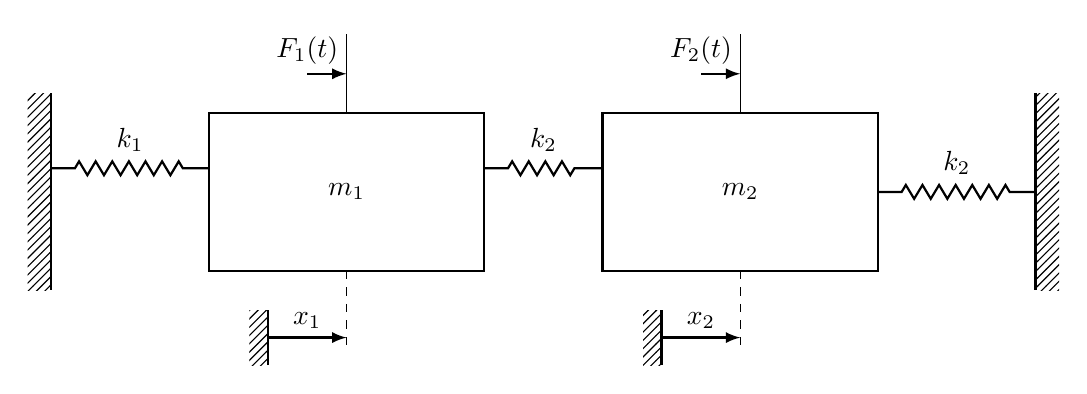
\begin{tikzpicture}[every node/.style={outer sep=0pt},thick,
    mass/.style={draw,thick},
    spring/.style={thick,decorate,decoration={zigzag,pre length=0.3cm,post
    length=0.3cm,segment length=6}},
    ground/.style={fill,pattern=north east lines,draw=none,minimum
    width=0.75cm,minimum height=0.3cm},
    dampic/.pic={\fill[white] (-0.1,-0.3) rectangle (0.3,0.3);
    \draw (-0.3,0.3) -| (0.3,-0.3) -- (-0.3,-0.3);
    \draw[line width=1mm] (-0.1,-0.3) -- (-0.1,0.3);}]

    \node[mass,minimum width=3.5cm,minimum height=2cm] (m1) {$m_1$};
    \node[mass,minimum width=3.5cm,minimum height=2cm,right=1.5cm of m1] (m2) {$m_2$};
    \node[left=2cm of m1,ground,minimum width=3mm,minimum height=2.5cm] (g1){};
    \draw (g1.north east) -- (g1.south east);
      \node[right=2cm of m2,ground,minimum width=3mm,minimum height=2.5cm] (g2){};
    \draw (g2.north west) -- (g2.south west);


    \draw[spring] ([yshift=3mm]g1.east) coordinate(aux) -- (m1.west|-aux) node[midway,above=1mm]{$k_1$};
    \draw[spring]  (m1.east|-aux) -- (m2.west|-aux) node[midway,above=1mm]{$k_2$};
    \draw[spring]  (m2.east) -- (g2.west) node[midway,above=1mm]{$k_2$};

    \foreach \X in {1,2}  
    {
      \draw[thin] (m\X.north) -- ++ (0,1) coordinate[midway](aux\X);
      \draw[latex-] (aux\X) -- ++ (-0.5,0) node[above]{$F_\X(t)$}; 
      \draw[thin,dashed] (m\X.south) -- ++ (0,-1) coordinate[pos=0.85](aux'\X);
      \draw[latex-] (aux'\X) -- ++ (-1,0) node[midway,above]{$x_\X$}
      node[left,ground,minimum height=7mm,minimum width=1mm] (g'\X){};
      \draw[thick] (g'\X.north east) -- (g'\X.south east);
    }
  \end{tikzpicture}
  \begin{enumerate}[label=(\alph*)]
    \item Derive the system of second order ordinary differential equations that describes the spring-mass system. 
    \item Write out the reduced system of ordinary differential equations in \textbf{vector form} that can be used to solve your system from part (a).
    \item Use the MATLAB function \texttt{ode45()} to solve your system from part (b) over time $[0, 200]$, with the following parameters:
    \begin{gather*}
      F_1(t) = \sin(t),~F_2(t) = e^{-t}\\
      k_1 = 2,~k_2 = 0.5\\
      m_1 = 3,~m_2 = 1
    \end{gather*}
  \end{enumerate}
}
\sol (a) \\
We have here 2 masses, $m_1$ and $m_2$, which are joined by 3 springs . The spring connected a fixed support to $m_1$ has spring constant $k_1$. The spring connecting $m_1$ to $m_2$ and $m_2$ to a fixed support, has spring constant $k_2$. An arbitrary push force $F_1$, itself a function of time, is applied to $m_1$. Another push force, $F_2$, also a function of time, is applied to $m_2$. These forces will cause $m_1$ and $m_2$ to be displaced from their equilibria, and these displacements are given by $x_1(t)$ and $x_2(t)$, respectively. \\

Newton's second law of motion states that the sum of all forces applied to an object is equal to the object's acceleration times its mass,
$$
  F = ma.
$$
Hooke's law states that the spring force is given by the spring's $k$-constant multipled by the distance from equilibrium,
$$
  F_s = kx
$$ 
Each mass has 2 springs acting on it, so each mass's net force is comprised of 3 forces: 2 spring forces, and 1 arbitrary push force. So, we can write
\begin{gather*}
  m_1a_1 = F_1 + F_{s1} + F_{s2} \\ 
  m_2a_2 = F_2 + F_{s3} + F_{s4}
\end{gather*}
\newpage
The spring force between the fixed surface and $m_1$ is acting against the displacing force. The spring between $m_1$ and $m_2$, in contrast, is contributing to the displacing force, relative to the displacement between the two masses. Therefore,
\begin{align*}
  F_{s1}(t) &= -k_1x_1(t) \\
  F_{s2}(t) &= k_2(x_2(t) - x_1(t)).
\end{align*}
The spring force between the $m_2$ and $m_1$ is acting against the displacing force, while the spring force between $m_2$ and the fixed surface acts along the displacement. Therefore,
\begin{align*}
  F_{s3}(t) &= k_2(x_1(t) - x_2(t)) \\
  F_{s4}(t) &= -k_2x_2(t)
\end{align*}
Finally, we note that acceleration, $a$, is the second derivative of position, $x$, with respect to time, $\ddot{x}$. Bringing this all together, we can describe the spring-mass system witth the following system of second-order differential equations,
\begin{align*}
  m_1\ddot{x}_1 &= F_1 - k_1x_1 + k_2(x_2 - x_1) \\ 
  m_2\ddot{x}_2 &= F_2 + k_2(x_1 - x_2) - k_2x_2
\end{align*}
Which we can simplify to
\begin{align*}
  m_1\ddot{x}_1 &= F_1 + (k_2 - k_1)x_1 + k_2x_2 \\ 
  m_2\ddot{x}_2 &= F_2 + k_2x_1 - 2k_2x_2
\end{align*}

\sol (b) \\
Let $v_1 = \dot{x}_1$ and $v_2 = \dot{x}_2$, and express the system we've derived in terms of these,
\begin{align*}
  m_1\dot{v}_1 &= F_1 + (k_2 - k_1)x_1 + k_2x_2 \\ 
  m_2\dot{v}_2 &= F_2 + k_2x_1 - 2k_2x_2
\end{align*}
Let $\ut{y}(t)$ be the state vector of the system,
$$
  \ut{y}(t) = \begin{pmatrix} x_1(t) \\ v_1(t) \\ x_2(t) \\ v_2(t) \end{pmatrix}.
$$
Taking the derivative,
$$
  \dd{t}\ut{y}(t) = \dd{t}\begin{pmatrix} x_1(t) \\ v_1(t) \\ x_2(t) \\ v_2(t) \end{pmatrix} = \begin{pmatrix} v_1(t) \\ \frac{1}{m_1}\bracks{F_1 + (k_2 - k_1)x_1 + k_2x_2} \\ v_2(t) \\ \frac{1}{m_2}\bracks{F_2 + k_2x_1 - 2k_2x_2} \end{pmatrix},
$$
which is the reduced vector form of the system we sought. \\

\sol(c) \\
\verb|PS4_script1.m| \hrule
\begin{lstlisting}{Matlab}
% Defining our given parameters
k1 = 2;
k2 = 0.5;
m1 = 3;
m2 = 1;
t_range = [0 200];
% The inital conditions
% Inital position and velocity are both 0
% i.e. The system starts at equilibrium
y0 = [0; 0; 0; 0];

% Defining the system, according to what we derived in the
% previous question. Note that y(1) = x_1(t), y(3) = x_2(t)
% and y(2) = v_1(t) = \dot{x}_1(t), y(4) = v_2(t) = \dot{x}_2(t). 
system = @(t, y) [
  y(2);
  (sin(t) + k2 * (y(3) - y(1)) - k1 * y(1)) / m1;
  y(4);
  (exp(-t) + k2 * (y(1) - y(3)) - 2 * k2 * y(3)) / m2;
];

[t, y] = ode45(system, t_range, y0);

% Plot the results. The displacement results are stored in
% y(:, 1 and 3). Whereas the velocity results are stored
% in y(:, 2 and 4). We'll plot and present the displacements
% of m_1 and m_2 over time. The question was a little vauge
plot(t, y(:, 1), 'b--', 'LineWidth', 1.5); hold on;
plot(t, y(:, 3), 'r-', 'LineWidth', 1.5);
set(gca, 'FontSize', 14);
box off;
title('Displacements of $m_1$ and $m_2$ for $t\in[0,200]$', ...
  'FontSize', 36, 'Interpreter', 'latex');
xlabel('Time $(t)$', 'FontSize', 36, 'Interpreter', 'latex');
ylabel('Displacement $(x_1, x_2)$', 'FontSize', 36, ...
  'Interpreter', 'latex');
legend('$x_1(t)$', '$x_2(t)$', 'FontSize', 36, ...
  'Interpreter', 'latex');
\end{lstlisting}
\verb|Output:|\\
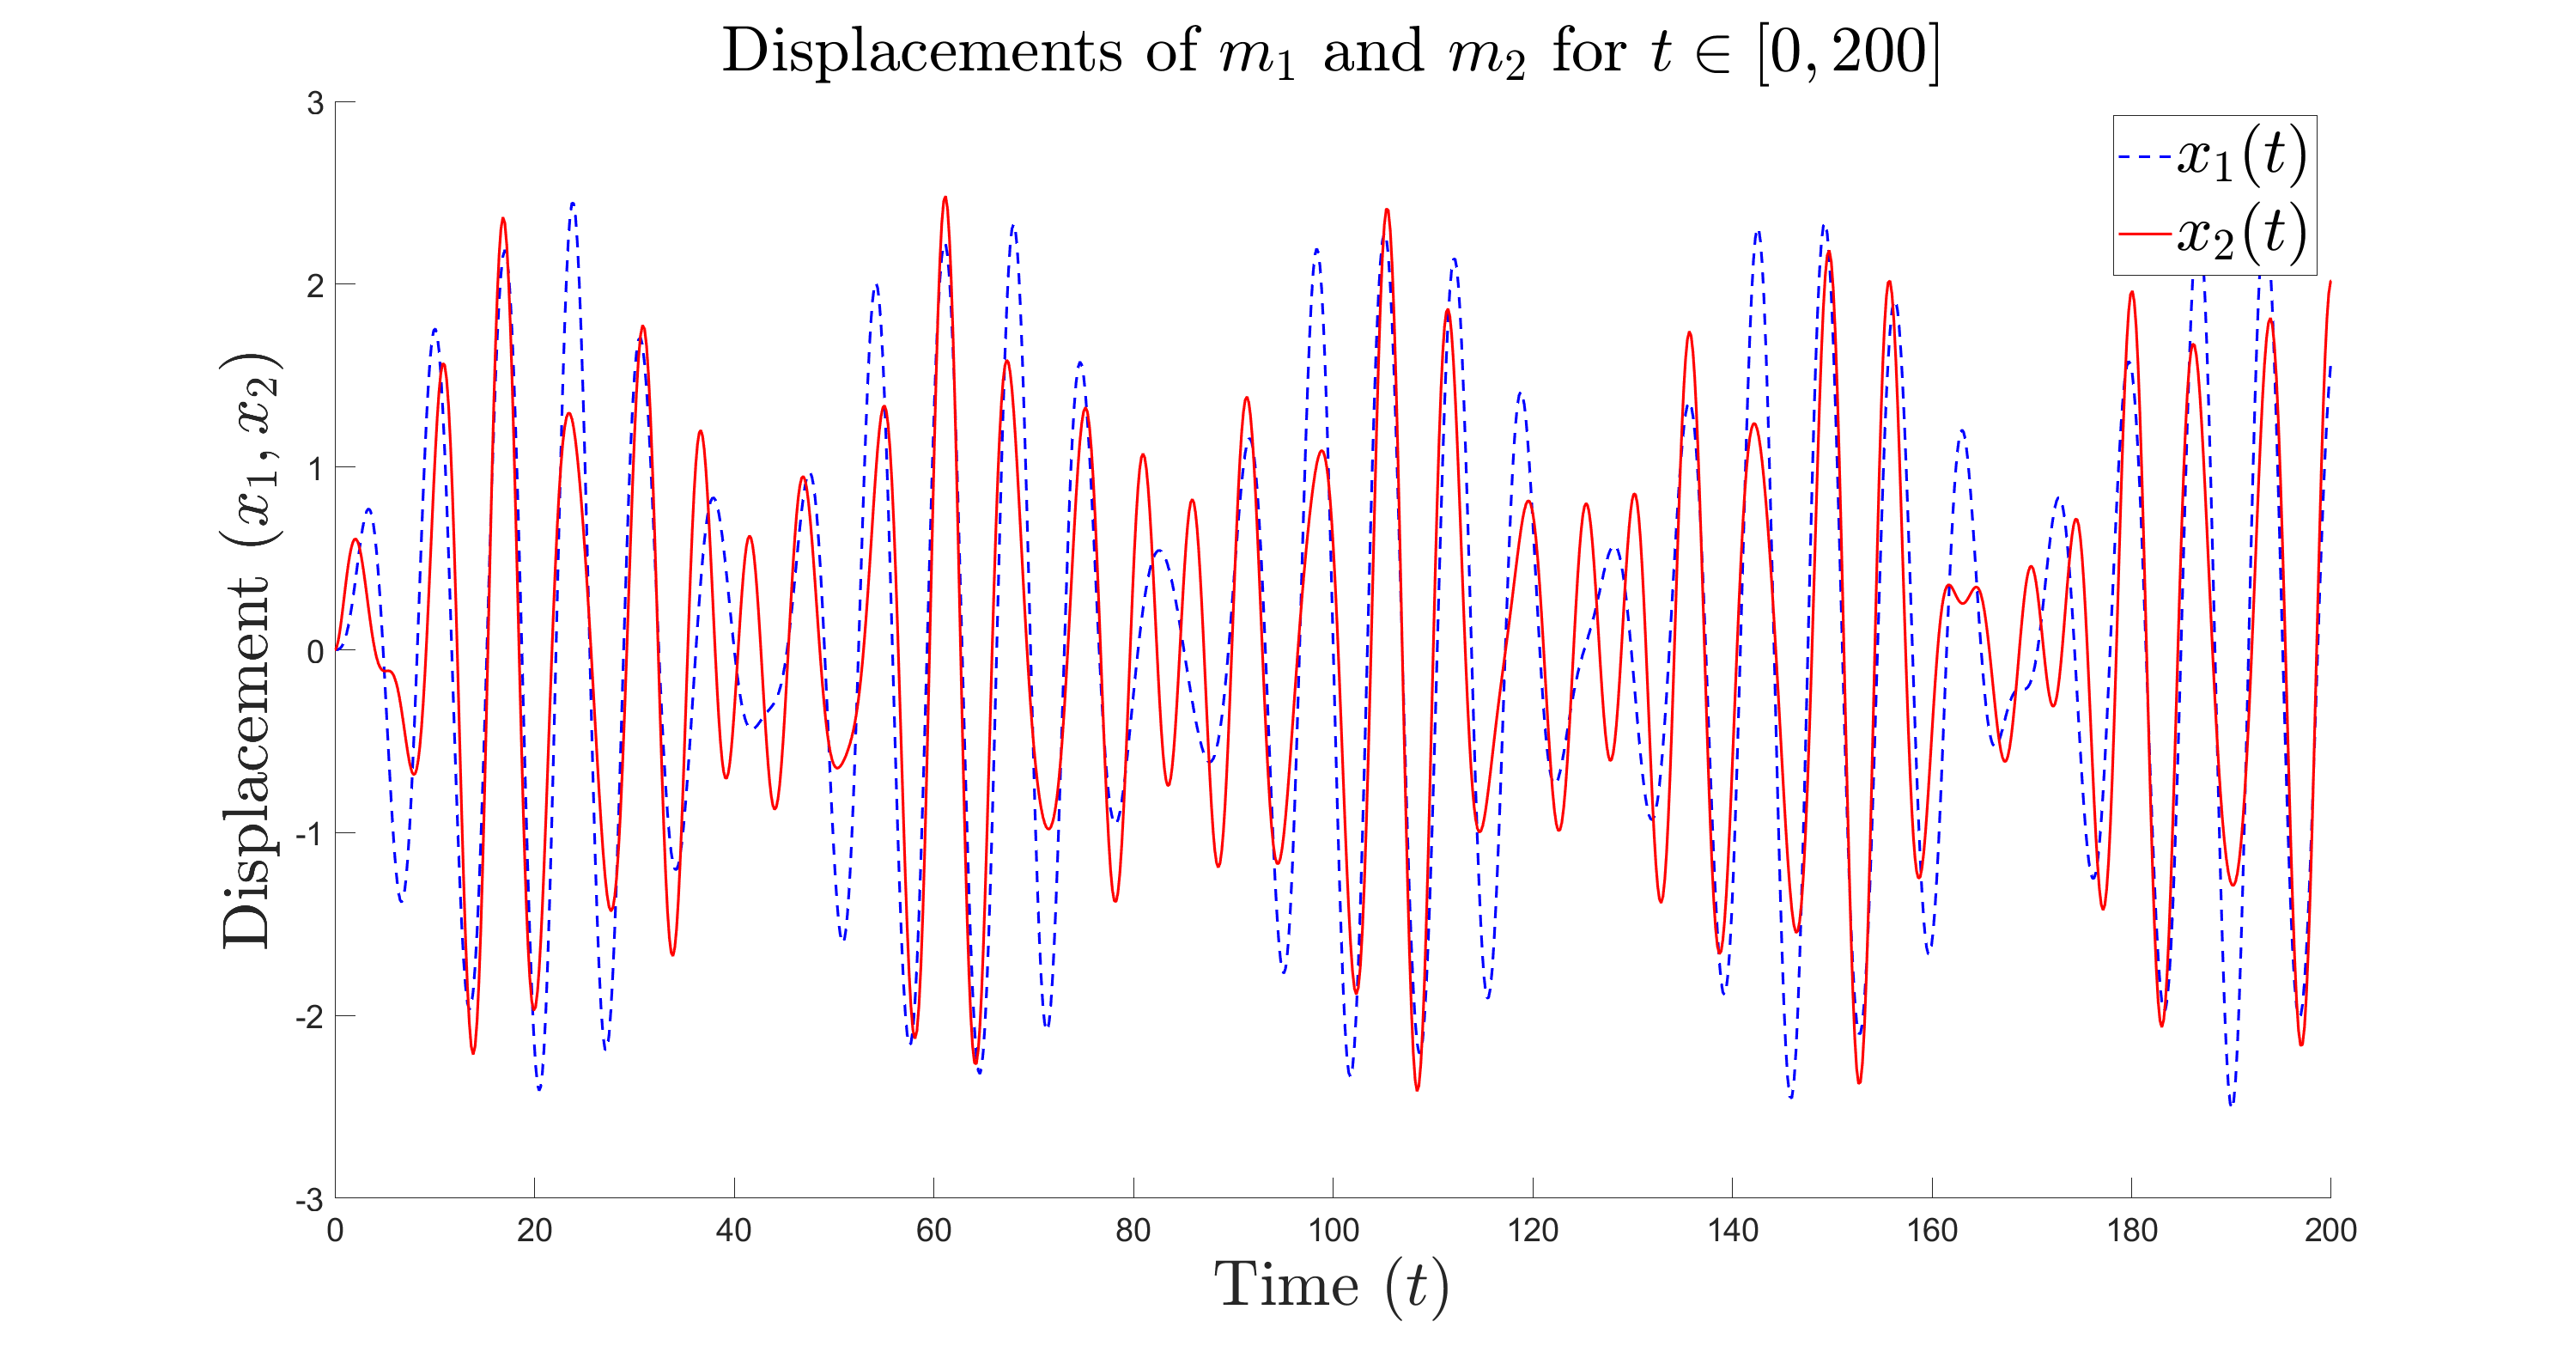
\includegraphics[width=\textwidth]{./PS4_fig1.png}

\newpage
\qs{}{
  We will explore what it means for the linear combination of solutions to a second-order differential equation, resulting from an application of the \textit{superposition principle}, to be a general solution to the corresponding initial value problem. That is, we will explore what it means for a set of solutions to form a \textbf{fundamental set of solutions}.
  \begin{enumerate}[label=(\alph*)]
    \item Suppose $y_1(t)$ and $y_2(t)$ are solutions to the second-order differential equation,
      $$
        p(t)y''+q(t)y'+r(t)y = 0.
      $$
      Use the superposition principle to find a general solution in terms of constant coefficients $c_1$ and $c_2$.
    \item Consider the initial conditions for the second-order differential equation given by,
      $$
        y(t_0) = y_0,~~~ y'(t_0) = y'_0.
      $$
      Apply these initial conditions to your solution from (a) and solve for the constants $c_1$ and $c_2$ using Cramer's rule: \\
      Given the system of linear equations, $\begin{bmatrix} a_1 & b_1\\ a_2 & b_2\end{bmatrix} \begin{bmatrix} c_1\\ c_2 \end{bmatrix} = \begin{bmatrix} y_0\\ y'_0 \end{bmatrix}$, then 
      $$
        c_1 = \frac{\begin{array}{|cc|} y_0 & b_1 \\ y'_0 & b_2 \end{array}}{\begin{array}{|cc|} a_1 & b_1 \\ a_2 & b_2\end{array}}\qquad 
        c_2 = \frac{\begin{array}{|cc|} a_1 & y_0\\ a_2 & y'_0 \end{array}}{\begin{array}{|cc|} a_1 & b_1 \\ a_2 & b_2\end{array}}
      $$
      where $|\cdot|$ denotes the determinant of the matrix. The quantity in the denominator is called the \textbf{Wronskian}.
    \item Use the Wronskian for $c_1$ and $c_2$ to develop a condition required for this initial value problem to be solvable. The set of solutions that satisfy this condition are called a \textbf{fundamental set of solutions}.
    \item Consider the second-order differential equation given by,
      $$
        2t^2 y''+ty'-3y = 0,~t>0.
      $$
      Given that $y_1(t) = t^{-1}$ is a solution to the second-order differential equation, find another solution $y_2(t)$ using the reduction of order method by assuming $y_2(t) = u(t)y_1(t)$. For ease of exposition, require that $u(1) = 0$ and $u'(1) = \frac{5}{2}$.
    \item Show that the solutions $y_1(t)$ and $y_2(t)$ form a fundamental set of solutions.
  \end{enumerate}
}
\sol (a) \\
By the superposition principle, the general solution to a homogenous second order differential equation, such as $y'' + p(t)y' + q(t) y = 0$, $y(t)$, is the sum of two linearly independent solutions, $y_1(t)$ and $y_2(t)$. The general solution is
\begin{gather*}
  y(t) = c_1y_1(t) + c_2y_2(t). \tag*{(1)}
\end{gather*}
So, transform the equation by dividing across by $p(t)$.
\begin{gather*}
  p(t)y'' + q(t)y' + r(t)y = 0 \\
  y'' + \frac{q(t)}{p(t)}y' + \frac{r(t)}{p(t)} y = 0
\end{gather*}
Now, because these are arbitrary functions of $t$, let 
\begin{align*}
  P(t) &= \frac{q(t)}{p(t)} & Q(t) &= \frac{r(t)}{p(t)}
\end{align*}
$$
\therefore y'' + P(t)y' + Q(t)y = 0
$$

This is now in a form where we can apply the superposition principle, and therefore the solution is the same as (1). \\

\sol (b) \\
Let's substitute the inital condition $y(t_0) = y_0$ into (1).
$$
  y(t_0) = c_1y_1(t_0) + c_2y_2(t_0) = y_0.
$$
Now, let's substitute the inital condition $y'(t_0) = y_0'$ into the derivative of (1).
$$
  y'(t_0) = c_1y_1'(t) + c_2y_2'(t) = y_0'.
$$
$$
  \text{Let}\left\lbrace \begin{array}{l} a_1 = y_1(t_0) \\ b_1 = y_2(t_0) \\ a_2 = y_1'(t_0) \\ b_2 = y_2'(t_0) \end{array} \right.\qquad\Then\left\lbrace \begin{array}{l} a_1c_1 + b_1c_2 = y_0 \\ a_2c_1 + b_2c_2 = y_0' \end{array} \right.
$$
which can be expressed as the linear system
$$
  \begin{pmatrix} a_1 & b_1 \\ a_2 & b_2 \end{pmatrix} \begin{pmatrix} c_1 \\ c_2 \end{pmatrix} = \begin{pmatrix} y_0 \\ y_0' \end{pmatrix}
$$
Applying Cramer's rule, and making back substitutions,
\begin{gather*}
  c_1 = \frac{\begin{array}{|cc|} y_0 & b_1 \\ y'_0 & b_2 \end{array}}{\begin{array}{|cc|} a_1 & b_1 \\ a_2 & b_2\end{array}} 
    = \frac{y_0b_2 - y_0'b_1}{a_1b_2 - a_2b_1} 
    = \frac{y_0y_2'(t_0) - y_0'y_2(t_0)}{y_1(t_0)y_2'(t_0) - y_1'(t_0)y_2(t_0)} \\
  c_2 = \frac{\begin{array}{|cc|} a_1 & y_0\\ a_2 & y'_0 \end{array}}{\begin{array}{|cc|} a_1 & b_1 \\ a_2 & b_2\end{array}}
    = \frac{a_1y_0' - a_2y_0}{a_1b_2 - a_2b_1}
    = \frac{y_0'y_1(t_0) - y_0y_1'(t_0)}{y_1(t_0)y_2'(t_0) - y_1'(t_0)y_2(t_0)}
\end{gather*}

\sol (c) \\
The second-order homogenous system is solvable if and only if the Wronskian of this system,
$$
  \begin{array}{|cc|} a_1 & b_1 \\ a_2 & b_2 \end{array} = y_1(t_0)y_2'(t_0) - y_1'(t_0)y_2(t_0) \neq 0.
$$
This condition is required, because if it isn't met, $c_1$ and $c_2$ are not defined, and hence there is no general solution to the homogenous second-order system of ODEs. \\

\sol (d) \\
Given that $y_1(t) = t^{-1}$ and $y_2(t) = u(t)y_1(t)$, we can see that
\begin{align*}
  y_2(t) &= u(t)t^{-1} \\
  \implies y_2'(t) &= u'(t)t^{-1} - u(t)t^{-2} \\
  \implies y_2''(t) &= u''(t)t^{-1} - 2u'(t)t^{-2} + 2u(t)t^{-3}
\end{align*}
We can substitute this solution back into the ODE, $2t^2y''+  ty' - 3y = 0,\ t>0$.
\begin{align*}
  2t^2y_2'' &= 2t^2\bracks{u''(t)t^{-1} - 2u'(t)t^{-2} + 2u(t)t^{-3}} = 2tu''(t) - 4u'(t) + 4u(t)t^{-1} \\
  ty_2' &= t\bracks{u'(t)t^{-1} - u(t)t^{-2}} = u'(t) - u(t)t^{-1} \\
  -3y_2 &= -3\bracks{u(t)t^{-1}} = -3u(t)t^{-1}
  \intertext{Now, we can express the system in terms of $u$ and its derivatives,}
  0 &= 2tu''(t) - 4u'(t) + 4u(t)t^{-1} +  u'(t) - u(t)t^{-1} - 3u(t)t^{-1} \\
    &= 2tu''(t) - 3u'(t)
  \end{align*}
If we let $v(t) = u'(t)$, we can rewrite this
$$
  2tv'(t) = 3v(t) \implies \frac{v'(t)}{v(t)} = \frac{3}{2t}
$$
Integrating both sides, we find that
$$
  \ln\abs{v(t)} = \frac{3}{2}\ln\abs{t} + C 
$$
Therefore
$$
  u'(t) = v(t) = C_1t^{3/2}
$$
Integrating again, we can find $u(t)$.
$$
  u(t) = \int C_1t^{3/2}\d{x} = \frac{2C_1}{5}t^{5/2} + C_2
$$
We can finally apply the given inital conditions and solve for the general solution of $u(t)$,
\begin{gather*}
  u(1) = 0 \implies 0 = \frac{2C_1}{5}(1)^{5/2} + C_2 = \frac{2C_1}{5} + C_2 \implies C_2 = -\frac{2}{5}C_1 \\
  u'(1) = \frac{5}{2} \implies \frac{5}{2} = C_1(1)^{3/2} = C_1 \implies C_1 = \frac{5}{2} \implies C_2 = -1 \\
  u(t) = \frac{2}{5}\cd\frac{5}{2}t^{5/2} - 1 = t^{5/2} - 1
\end{gather*}
Now, we can substitute this $u(t)$ back into our solution for $y_2(t)$,
$$
  y_2(t) = u(t)t^{-1} = \bracks{t^{5/2} - 1}t^{-1} = t^{3/2} - t^{-1}.
$$

\sol (e) \\
This $y_1$ and $y_2$ form a fundamental set of solutions if and only if they are linearly independent, if and only if their Wronskian is greater then 0 for all $t$.
$$
  \begin{array}{|cc|} y_1(t) & y_2(t) \\ y_1'(t) & y_2'(t) \end{array}
    = \begin{array}{|cc|} t^{-1} & t^{3/2} - t^{-1} \\ -t^{-2} & \frac{3}{2}t^{1/2} + t^{-2} \end{array} 
    = \frac{3}{2}t^{-1/2} + t^{-3} + t^{-1/2} - t^{-3}
    = \frac{5}{2}t^{-1/2}
    = \frac{5}{2\sqrt{t}}
$$
For all $t>0$, $\frac{5}{2}t^{-1/2}\neq0$. We know this is true, because as $t$ approaches 0 from the right side (the only side from which it could approach, by definition) $\frac{5}{2}t^{-1/2}$ goes to infinity. As $t$ goes to infinity, $\frac{5}{2}t^{-1/2}$ asymptotically approaches $0$, but never gets there. Therefore, this $y_1$ and $y_2$ form a fundamental set of solutions.

\clearpage
\qs{Second-Order Inhomogeneous DE}{
  Solve the following initial value problem for the second-order inhomogeneous differential equation,
  $$
    y''-4y'-12y = 2e^{5t},\ y(0) = \frac{8}{7},\ y'(0) = -\frac{1}{7}.
  $$
}
\sol The general solution for this IVP will take the form
$$
  y(t) = y_h(t) + y_p(t),
$$
where $y_h$ and $y_p$ are solutions to some homogenous and particular equation, respectively.
\begin{gather*}
  y_h(t) = \e{\lm t},\quad \text{for some}\ \lm\in\bbr. \\
  \Then {y_h}'(t) = \lm\e{\lm t}\quad \text{and}\quad {y_h}''(t) = \lm^2\e{\lm t}. \\
  \So \lm^2\e{\lm t} - 4\lm\e{\lm t} - 12\e{\lm t} = 0\ \text{is a homogenous equation we can solve.} \\
  \begin{align*}
    \bracks{\lm^2 - 4\lm - 12}\e{\lm t} &= 0.
    \intertext{Since $\forall x\in\bbr,\ \e{x} > 0$, and $\lm t\in\bbr$, we can safely through divide by $\e{\lm t}$.}
    \Hence \lm^2 - 4\lm - 12 &= 0, \\
    \Rightarrow (\lm-6)(\lm+2) &= 0. \\
    \tf \lm &\in \braces{-2, 6}.
  \end{align*}
  \intertext{Therefore the solution to the homogenous equation, by the superposition principle, is the sum of these two solutions,}
  \Rightarrow y_h(t) = \alpha\e{-2t} + \beta\e{6t}.
  \longintertext{Since, $y'' - 4y' - 12y = 2\e{5t}$, we can safely assume a particular solution $y_p(t)=A\e{5t}$.}
  \Rightarrow y_p'(t) = 5A\e{5t} \quad\text{and}\quad y_p''(t) = 25A\e{5t}.
  \intertext{Let's now substitute $y_p(t)$ and its derivatives back into the original inhomogeneous equation.}
  \begin{aligned}
    \bracks{25A\e{5t}} - 4\bracks{5A\e{5t}} - 12\bracks{A\e{5t}} &= 2\e{5t} \\
    25A\e{5t} - 20A\e{5t} - 12A\e{5t} &= 2\e{5t} \\
    \bracks{25A - 20A - 12A}\e{5t} &= 2\e{5t} \\
    -7A\e{5t} &= 2\e{5t} \\
    -7A &= 2 \\
    A &= -\frac{2}{7} \\
    \tf y_p(t) &= -\frac{2}{7}\e{5t}
  \end{aligned}
  \intertext{Substituting the $y_p$ and $y_h$ we've found back into the general solution $y(t)$,}
  \begin{align*}
    y(t) &= y_h(t) + y_p(t) \\
      &= \alpha\e{-2t} + \beta\e{6t} - \frac{2}{7}\e{5t}.
    \intertext{Into the general solution now, substitute the inital condition, $y(0)=\frac{8}{7}$.}
    \frac{8}{7} &= \alpha\e{-2\cd0} + \beta\e{6\cd0} - \frac{2}{7}\e{5\cd0} \\
      &= \alpha\e{0} + \beta\e{0} - \frac{2}{7}\e{0} \\
      &= \alpha + \beta - \frac{2}{7} \\
    \tf\alpha + \beta &= \frac{8}{7} + \frac{2}{7} = \frac{10}{7} \tag*{(1)} \\
    \intertext{Take the derivative of the general solution,}
    y'(t) &= \dd{t}\bracks{\alpha\e{-2t} + \beta\e{6t} - \frac{2}{7}\e{5t}} \\
      &= -2\alpha\e{-2t} + 6\beta\e{6t} - \frac{10}{7}\e{5t}.
    \intertext{Now substituting the inital condition, $y'(0)=-\dfrac{1}{7}$,}
    -\frac{1}{7} &= -2\alpha\e{-2\cd0} + 6\beta\e{6\cd0} - \frac{10}{7}\e{5\cd0} \\
      &= -2\alpha\e{0} + 6\beta\e{0} - \frac{10}{7}\e{0} \\
      &= -2\alpha + 6\beta - \frac{10}{7}. \\
    \tf -2\alpha + 6\beta &= -\frac{1}{7} + \frac{10}{7} = \frac{9}{7} \tag*{(2)}
  \end{align*}
  \intertext{We will now solve the linear system, $A\ut{x}=\ut{b}$, formed by (1) and (2),}
  A\ut{x}=\ut{b} := \begin{pmatrix} 1 & 1 \\ -2 & 6 \end{pmatrix}\begin{pmatrix} \alpha \\ \beta \end{pmatrix} = \begin{pmatrix} 10/7 \\ 9/7 \end{pmatrix}. \\
  \rightsquigarrow \left( \begin{array}{cc|c} 1 & 1 & 10/7 \\ -2 & 6 & 9/7 \end{array}\right)
  \rightsquigarrow \left( \begin{array}{cc|c} 1 & 1 & 10/7 \\ 1 & -3 & -9/14 \end{array}\right)
  \rightsquigarrow \left( \begin{array}{cc|c} 1 & 1 & 10/7 \\ 0 & -4 & -29/14 \end{array}\right)\\
  \rightsquigarrow \left( \begin{array}{cc|c} 1 & 1 & 10/7 \\ 0 & 1 & 29/56 \end{array}\right)
  \rightsquigarrow \left( \begin{array}{cc|c} 1 & 0 & 51/56 \\ 0 & 1 & 29/56 \end{array}\right)
  \implies \bracks{\alpha,\beta} = \bracks{\frac{51}{56}, \frac{29}{56}}.
  \intertext{Finally, let's substitute $\alpha$ and $\beta$ back into the gernal solution, and present our final solution.}
  y(t) = \frac{51}{56}\e{-2t} + \frac{29}{56}\e{6t} - \frac{2}{7}\e{5t}.
\end{gather*}

\end{document}
